\documentclass[../main.tex]{subfiles}

\begin{document}

\chapter[Resilient Primal Decomposition-based dMPC]{Resilient \\Primal Decomposition-based \\distributed \\Model Predictive Control}\label{sec:safe_pddmpc_ineq}
\epigraph{\centering Desperate times call for desperate measures}
{\textit{Title}\\\textsc{Author}}

In this chapter, we carry on the work from the last chapter relaxing some assumptions to make the problem to be solved more generic.
We apply the primal decomposition to the problem, and then, we compare the cases when the system presents nominal behavior and when the system is under the proposed attack model.

From the analysis, we notice how the relaxation of the assumption increases drastically the complexity of the problem.

Employing some assumptions, we take a powerful tool of our identification utility belt, and use it to create an approach to circumvent the complexity of the system, allowing us to adapt the detection and mitigation presented in the last chapter.

\minitoc

\section{Relaxing the problem}\label{sec:not-so-scarce}
We begin again with the monolithic \mpc{} equivalent problem~\eqref{eq:qp_standard_form}.
We reproduce yet another time the problem, but with a twist, now the problem also has a decomposable constraint set $\set{U}$:
\begin{equation}
  \label{eq:qp_standard_form_again_set_constraint}
  \begin{aligned}
    \begin{matrix}
      \minimize\limits_{\vec{U}[k]} &
                                                 \frac{1}{2}\norm{\vec{U}[k]}^{2}_{H} + {\vec{f}[k]}^{T}\vec{U}[k] &\\
      \mathrm{subject~ to} & \bar{\Gamma}\vec{U}[k]\preceq {\vec{U}}_{\text{max}} \\
                                    & \vec{U}[k]\in \set{U}
    \end{matrix}
  \end{aligned}.
\end{equation}
We decompose the system using the primal decomposition, and the local problems also have constraint sets, denoted $\set{U}_{i}$:
\begin{equation}
  \label{eq:DOP_local_set_constraint}
  \eqoptobji(\thetaik)[k]=
  \begin{matrix}
    \minimize\limits_{\vec{U}_{i}[k]}&\frac{1}{2}\norm{\vec{U}_{i}[k]}^{2}_{H_{i}} + {\vec{f}_{i}[k]}^{T}\vec{U}_{i}[k]\\
    \mathrm{subject~ to} & \bar{\Gamma}_{i}\vec{U}_{i}[k] \preceq \thetaik:\lambdaik\\
    & \vec{U}_{i}[k]\in \set{U}_{i}
  \end{matrix},
\end{equation}
and we use the projected subgradient method~\eqref{eq:projectedSubgradient_lambda} (reproduced for convenience) to solve the main problem:
\begin{equation}
  \label{eq:projectedSubgradient_lambda_reprise}
  \tag{\ref*{eq:projectedSubgradient_lambda}}
  \vec{\theta}[k]\pplusone=\Proj^{\set{S}}(\vec{\theta}[k]\p+\rho\p\vec{\lambda}[k]\p),
\end{equation}
but with ${\set{S} = \setbuild{\vec{\theta}[k]}{I_{c}^{M}\vec{\theta}[k]\preceq \vec{U}_{\max}}}$.
\begin{remark}
  As seen in~\cite{BoydEtAl2015}, if we have separable constraints sets, such as the $\set{U}_{i}$ in our problem, we can modify the local objectives $\obji$ so \begin{equation*}
    J_{i}(\optthetai)=\infty\text{, if }\vec{U}_{i}^{\star}\notin\dom{\obji}.
  \end{equation*}
  Since this change modifies the objective functions, it also modifies the corresponding gradients, and $\lambdai$ as consequence.
  So, this change guides the coordinator to choose $\thetai$ which respect $\dom{\obji}$.
\end{remark}

In this chapter, we still assume the original constraint~\eqref{eq:linear_constraint} to have at most as many rows as columns, i.e., $\card{\vec{u}_{\max}}\leq n_{u}$.
However, we relax the assumption made in \S\ref{sec:scarce-systems}.
The systems are not necessarily scarce anymore, i.e., the unconstrained solutions
$\optuncU=-H^{-1}\vec{f}[k]$ and $\optuncUik=-H_{i}^{-1}\vec{f}_{i}[k]$ may or may not respect the constraints.

As we will see in next section, despite the relaxation of this assumption, making the problem more generic, it causes the solution of the local problems exponentially more complex.

\todo{Nonetheless, to assure some properties we make another assumption, we assume the unconstrained solutions respect the constraint sets,\note{where to put this?? Maybe when discussing artificial scarcity}
\begin{align}
  \optuncU\in\set{U}\\
  \optuncUik\in\set{U}_{i}.
\end{align}
}

\section{Impact on local problems' solution}\label{sec:impact-local-problem}
We can repeat the analysis made in the last chapter to see how the change on assumption influences the solutions of the problem.

Although now we have \qp{} problems with inequality constraints, we still can use the same method to find a analytical solution.

We similarly define a function $\inequalityfunctionname:\R^{\card\vec{U}_{i}[k]}\times \R^{\card\thetaik}$:
\begin{equation}
  \label{eq:lagrangian_inequality}
  \inequalityfunction=\bar{\Gamma}_{i}\vec{U}_i[k]-\thetaik,
\end{equation}
and use it to put the problem in standard form for inequality constraint \qp{} programs:
\begin{equation}
  \begin{matrix}
  \label{eq:local_problem_equality_standard_notation}
    \minimize\limits_{\vec{U}_{i}[k]}&\obji(\vec{U}_{i}[k],\thetaik)\\
    \mathrm{subject~ to} & \inequalityfunction\preceq 0:\lambdaik
  \end{matrix},
\end{equation}
with variables $\lambdaik$ associated to the constraints.
\begin{remark}
  Usually we make the distinction between the dual variables associated to the inequality and equality constraints by using different symbols.
  However, as in the problems we have only one kind, we use the same symbol and by context the reader can distinguish to which kind the symbol corresponds.
\end{remark}

We can again define the \emph{Lagrangian} function $\lagrangianname : \R^{\card\vec{U}_{i}[k]}\times \R^{\card\lambdaik} \times \R^{\card\thetaik} \to \R$ as
\begin{equation}
  \label{eq:lagrangian_equality}
  \lagrangian=\obji(\vec{U}_{i}[k],\thetaik)+\lambdaik^T\inequalityfunction,
\end{equation}
which embeds the inequality constraint into the objective function using $\lambdaik$, in this case the lagrangian multiplier for \emph{inequality}.
Again, since there is only one type of lagrangian multiplier, we will call it simply as the dual variable.

\begin{remark}
  The complementary slackness still holds, ${\lambdaikstar}^T\inequalityfunctionname(\vec{U}_{i}^{\star}[k],\thetaik)$ will always be zero.
  If any element of $\inequalityfunctionname(\vec{U}_{i}^{\star}[k],\thetaik)$ is smaller than zero, the corresponding element on the dual variable $\lambdaikstar$ will be zero, indicating the constraint is active.
\end{remark}

We can define the dual function $\dualfunctionname:\R^{\card\lambdaik} \times \R^{\card\thetaik} \to \R$ also calculated by solving
\begin{equation}
  \label{eq:dual_function_equality}
  \dualfunction=\inf_{\vec{U}_{i}[k]\in\set{F}} \lagrangian,
\end{equation}
but now where $\set{F}=\dom \inequalityfunctionname=\bigcap\limits_{i=1}^{\card\vec{U}_{\max}}\set{H}_{i}$, with $\set{H}_{i}$ being the halfspaces
${\set{H}_i=\setbuild{\vec{x}}{\elem[i,\star]{{\bar{\Gamma}}}\vec{x}\leq\elem[i,\star]{\vec{U}_{\max}}}}$.
Using the first order \KKT{} optimality condition we have
\begin{equation}
\nabla_{\vec{U}_{i}[k]}\lagrangian=0
\end{equation}
yielding as well
\begin{equation}
\vec{U}_{i}[k]=-H_{i}^{-1}\vec{f}_{i}[k]+H_{i}^{-1}\bar{\Gamma}_{i}^{T}\lambdaik,
\end{equation}
which we know is
\begin{equation}
\vec{U}_{i}[k]=\optuncUik-H_{i}^{-1}\bar{\Gamma}_{i}^{T}\lambdaik.
\end{equation}

Substituting it in $\lagrangian$ results
\begin{equation}
  \label{eq:dual_function_solution_lambda_theta_ineq}
\dualfunction=-\frac{1}{2}\lambdaik^{T}\linearcoefi\lambdaik-\lambdaik^{T}\bar{\Gamma}_{i}H_{i}^{-1}\vec{f}[k]-\lambdaik^{T}\thetaik,
\end{equation}
which is also concave.

Then, similarly we can find $\lambdaikstar$ by solving an optimization problem.
However, since we are using inequalities, we can only have $\lambdaik$ positive~\cite{BoydVandenberghe2004}:
\begin{equation}
  \label{eq:ineq_lambda_equation}
  \begin{matrix}
    \lambdaikstar=\argmax\limits_{\lambdaik}\left\{
    \begin{matrix}
    \maximize\limits_{\lambdaik}&\dualfunction\\
      \mathrm{subject~ to}& \lambdaik\preceq\0
    \end{matrix}\right\}.
  \end{matrix}
\end{equation}

As we know, by complementary slackness, the value of the elements of $\lambdaik$ being $0$ (or different of $0$) will depend on the status of the corresponding constraint for the unconstrained solution $\optuncUik$.
So the complete value of $\lambdaik$ will depend of the permutation of the status of the inequality constraint.
Depending on the form of the constraints, if we have $\nineq$ constraints, we may have potentially $2^{\nineq}$ permutations.
\begin{remark}
  Here we say potentially because not necessarily all combinations are possible.
  In \S\ref{sec:cons-about-stat} we discuss briefly about the number of permutations and show some cases where the number of permutations is not equal to $2^{\nineq}$.
\end{remark}

To solve~\eqref{eq:ineq_lambda_equation}, we can use the fact that the status of the constraints depends on the value of $\thetaik$.
This way, we can notice that the set of constraints divides the space of $\thetaik$ into multiple regions, depending if the constraints are active or not for $\optuncUik$.

$\optuncUik$
$\optuncU$

Imagine an example where we have $2$ constraints with associated $\elem[1]{\lambdai}$ and $\elem[2]{\lambdai}$, the $\thetai$ solution space is partitioned like in Fig.~\ref{fig:constraints_partition_theta} (indices $[k]$ suppressed for brevity).
\begin{figure}[h]
\centering
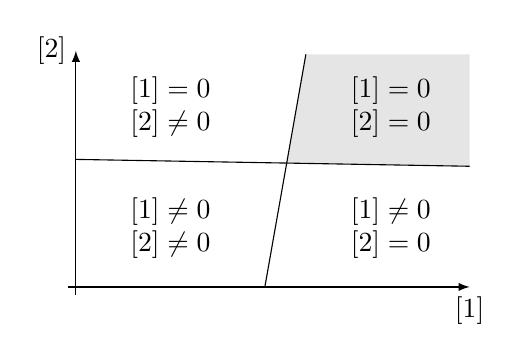
\begin{tikzpicture}[every node/.style={align=center}]
\def\height{3}
\def\length{5}
\node at (0,0) {} coordinate (p0)  ++(0:\length*2.4/5) coordinate (p1) ;
\node at (0,0) {} ++(90:\height*2.7/5) coordinate (p2) ;

\draw[black] (p2) ++(-1:5) coordinate (p3);
\draw[black] (p1) ++(80:3) coordinate (p4);
\coordinate (p6) at (p3|-p4);

\coordinate (p5) at (intersection cs:first line={(p2)--(p3)}, second line={(p1)--(p4)});
\path[fill=gray!20] (p6) -- (p4) -- (p5) -- (p3);
\draw[black] (p2) -- (p3);
\draw[black] (p1) -- (p4);

\draw[-latex] (0,-.1) - - (0,\height) node[left]{$\elem[2]{\thetai}$};
\draw[-latex] (-.1,0) - - (\length,0) node[below]{$\elem[1]{\thetai}$};

\node at (\length*1.2/5,\height*1.25/5) {$\elem[1]{\lambdai}\neq0$\\$\elem[2]{\lambdai}\neq0$};
\node at (\length*1.2/5,\height*3.8/5) {$\elem[1]{\lambdai}=0$\\$\elem[2]{\lambdai}\neq0$};
\node at (\length*4/5,\height*1.25/5) {$\elem[1]{\lambdai}\neq0$\\$\elem[2]{\lambdai}=0$};
\node at (\length*4/5,\height*3.8/5) {$\elem[1]{\lambdai}=0$\\$\elem[2]{\lambdai}=0$};
\end{tikzpicture}
\caption{Constraints partitioning $\thetai$ solution space.}\label{fig:constraints_partition_theta}
\end{figure}
For any $\thetai$ inside the grey area, the solution to~\eqref{eq:local_problem_equality_standard_notation} will be unconstrained, i.e., the constraint will be active.
Thus, for this case, by definition the value of $\lambdai=\0$.
For all other cases, where we know at least one constraint in~\eqref{eq:local_problem_equality_standard_notation} is inactive, we can remove the constraint in~\eqref{eq:ineq_lambda_equation} for the element of $\lambdai$ corresponding to the inactive constraint.
For instance, if all constraints in~\eqref{eq:local_problem_equality_standard_notation} are inactive, we can remove all constraints of~\eqref{eq:ineq_lambda_equation}, which will result in problem~\eqref{eq:eq_lambda_equation}, whose solution we known already:
\begin{equation}
  \label{eq:lambda_function_theta_reprise}
  \tag{\ref*{eq:lambda_function_theta}}
  \lambdaik=-\Plin\thetaik-\sik,
\end{equation}
\newcommand{\Plinineqnonzero}[1][\star]{\overset{#1}{\Plin}}
\newcommand{\sikineqnonzero}[1][\star]{\overset{#1}{\vec{s}_{i}}[k]}

By removing a set of constraints, we can solve a similar problem, but with reduced number of elements in $\thetai$ and $\lambdai$.
For example, let us suppose the first constraint in~\eqref{eq:local_problem_equality_standard_notation} is active.
We make $\elem[1]{\lambdai}=0$ and set it aside, we remove the corresponding lines of $\bar{\Gamma}_{i}$ and $\thetai$, and then we solve for all other elements of $\lambdai$, removing the remaining constraints in~\eqref{eq:ineq_lambda_equation}. This results in
\begin{equation}
  \label{eq:lambda_function_theta_some_active}
  \elem[2:\elemend]{\lambdai}[k]=-\Plinineqnonzero[2:\card{\lambdai}] \elem[2:\elemend]{\thetai}[k]-\sikineqnonzero[2:\card{\lambdai}],
\end{equation}
where $\Plinineqnonzero[2:\card{\lambdai}]={(\linearcoefiineqnonzero[2:\elemend,\star])}^{-1}$ and $\sikineqnonzero[2:\card{\lambdai}]=\Plinineqnonzero[2:\card{\lambdai}]\elem[2:\elemend,\star]{\bar{\Gamma}_{i}}H_{i}^{-1}\vec{f}_{i}[k]$.

If we do this for all partitions, i.e., all possible permutations of active and inactive constraints, we will have as many equations similar to~\eqref{eq:lambda_function_theta_some_active} as permutations.
This result is the base for calculating the solution of the original problem~\eqref{eq:local_problem_equality_standard_notation} as shown in~\cite{BemporadEtAl2002,AlessioBemporad2009}, which is the base for explicit \mpc{}.

However, the equations have different sizes of elements (as many elements as inactive constraints).
To make all equations same-sized, we recover the elements of $\lambdai$ set to zero and set aside.
If we take the same example, Eq.~\eqref{eq:lambda_function_theta_some_active} would become
\begin{equation}
  \label{eq:lambda_function_theta_some_active_same_size}
  \lambdaik=
  \left[
    \begin{matrix}
      0\\
      \elem[2:\elemend]{\lambdai}[k]
    \end{matrix}
  \right]
  =
  -
  \left[
    \begin{matrix}
      0&0\\
      0&\Plinineqnonzero[2:\card{\lambdai}]
    \end{matrix}
  \right]
  \thetaik
  -
  \left[
    \begin{matrix}
      0\\
      \sikineqnonzero[2:\card{\lambdai}]
    \end{matrix}
  \right]
\end{equation}


To facilitate the notation, let's use a binary representation such if we have $\nineq$, we use $\nineq$ binary digits to represent the active constraints.
And we will mark the digtis $1$ if the constraint is active and $0$ if inactive, indicating which constraints were removed or kept.

If we retake the $2$-constraints example in Fig.~\ref{fig:constraints_partition_theta}, ${00}_{(2)}$ would represent both constraints inactive (bottom left quadrant), ${01}_{(2)}$ and ${10}_{(2)}$ represents one of the constraints are active (bottom right and top left quadrants, respectively) and ${11}_{(2)}$ where both constraints are active (grey area in top right quadrant).
We can then use the base 10 to represent such partitions.
This way~\eqref{eq:lambda_function_theta_some_active_same_size} can be written as
\begin{equation}
  \label{eq:lambda_function_theta_same_size_coded}
  \lambdaik=-\Plin^{(2^{n_{\text{ineq}-1}})}\thetaik-\sik^{(2^{n_{\text{ineq}-1}})},
\end{equation}
with index $(2^{n_{\text{ineq}-1}})$ indicating that only the first constraint is active.

Then, we can write the complete solution of~\eqref{eq:ineq_lambda_equation} as
a \pwa{} function
\begin{equation}
  \label{eq:lambdafuntheta}
  \begin{aligned}
    \lambdaik=
    \begin{cases}
      -\Plinineq\thetaik-\sikineq,&\text{if}\ G^{0}[k]\thetaik \preceq b^{0}[k] \\
      \qquad\quad \vdots&\qquad\quad \vdots\\
      -\Plinineq[i][2^{\nineq}-1]\thetaik-\sikineq[i][2^{\nineq}-1],&\text{if}\ G^{2^{\nineq}-1}[k]\thetaik \preceq b^{2^{\nineq}-1}[k] \\
    \end{cases}
  \end{aligned}
\end{equation}
with halfspaces defined by the pairs $(G^{n}[k],\vec{b}^{n}[k])$ representing the partitions of the solution space which may vary with time $k$.
\begin{remark}
  Determining the exact halfspaces is not in the scope of this work.
\end{remark}

Here we can begin to regard the change caused by the relaxation, whereas we had only one equation relating $\lambdai$ to $\thetai$, when the system was scarce, now we have potentially $2^{\nineq}$ different equations.

\begin{remark}\label{rem:sparse_solutions}
  As one may expect, by definition, the $\Plinineq[i][n]$ and $\sikineq[i][n]$ are increasingly sparse, as $n$ increases more constraints are active and more blocks are equal to zero, culminating in $\Plinineq[i][2^{\nineq}-1]=0_{\card{\lambdai}}$ and $\sikineq[i][2^{\nineq}-1]=\0_{\card{\lambdai}}$.
\end{remark}
\subsection{Considerations about status of constraints}\label{sec:cons-about-stat}
It is important to observe that some there are some sets of constraints in which the permutation is not necessarily $2^{\nineq}$.

For example, in some cases there is no partition where all constraints are active, i.e., the intersection of halfspaces is empty (see Fig.~\ref{fig:non_feasible}).
Problems with such constraints are infeasible, thus we ignore them in this work.

\begin{figure}[H]
  \centering
  \begin{tikzpicture}
    \def\ang{-35}
    \def\vecmag{.25}
    \node at (0,0) {} coordinate(p1) ++(\ang:2.5) coordinate(p2) ++(\ang-90:1.5) coordinate(p3) ++(\ang-180:2.5) coordinate(p4);

    \path (p1) -- (p2) coordinate[pos=-0.2](a1l) coordinate[pos=1.2](a1r) coordinate[pos=0.8](m12);
    \draw[-latex] (a1l) -- (m12) -- ([turn] -90:0.5) node[left]{$\vec{\eta}_1$};
    \draw  (m12) -- (a1r);

    \path (p3) -- (p4) coordinate[pos=-0.2](a3l) coordinate[pos=1.2](a3r) coordinate[pos=0.8](m34);
    \draw[-latex] (a3l) -- (m34) -- ([turn] -90:0.5) node[right]{$\vec{\eta}_2$};
    \draw  (m34) -- (a3r);

  \end{tikzpicture}
  \caption{Set of constraints with no intersection.}\label{fig:non_feasible}
\end{figure}

In other cases, there is no combination where all constraints are inactive.
We give some different examples.
For instance, for constraints with normals $\vec{\vec{\eta}}_{i}$, if the angles of adjacent halfspaces $\vecangle{\vec{\eta}_{i}}{\vec{\eta}_{j}}$ is $180^{o}$ and the intersection is not nil (see Fig.~\ref{fig:parallel_only_one_active}), one of the constraints will always be active.
\begin{figure}[H]
  \centering
  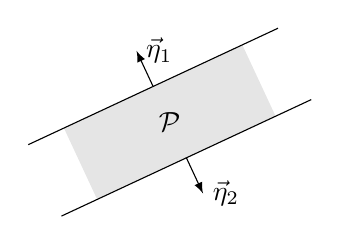
\begin{tikzpicture}
    \def\ang{25}
    \def\vecmag{.5}
    \node at (0,0) {} coordinate(p1) ++(\ang:2.5) coordinate(p2) ++(\ang-90:1.) coordinate(p3) ++(\ang-180:2.5) coordinate(p4);
    \path[fill=gray!20] (p1) -- (p2) -- (p3) -- (p4);
    \node at (barycentric cs:p1=1,p2=1,p3=1,p4=1) {$\mathcal{P}$};

    \path (p1) -- (p2) coordinate[pos=-0.2](a1l) coordinate[pos=1.2](a1r) coordinate[pos=0.5](m12);
    \draw[-latex] (a1l) -- (m12) -- ([turn] 90:0.5) node[right]{$\vec{\eta}_1$};
    \draw  (m12) -- (a1r);

    \path (p3) -- (p4) coordinate[pos=-0.2](a3l) coordinate[pos=1.2](a3r) coordinate[pos=0.5](m34);
    \draw[-latex] (a3l) -- (m34) -- ([turn] 90:0.5) node[right]{$\vec{\eta}_2$};
    \draw  (m34) -- (a3r);
  \end{tikzpicture}
  \caption{Two constraints with $\vecangle{\vec{\eta}_{1}}{\vec{\eta}_{2}}=180^{o}$.}\label{fig:parallel_only_one_active}
\end{figure}

Yet another example, are when the constraints form a convex polyhedron.
We present a minimal example of polyhedron in Fig.~\ref{fig:triangle_inequality}, a triangle in $\R^{2}$ formed by $3$ inequality constraints.
In this case, there will always be at least $2$ active constraints.
\begin{figure}[h]
  \centering
  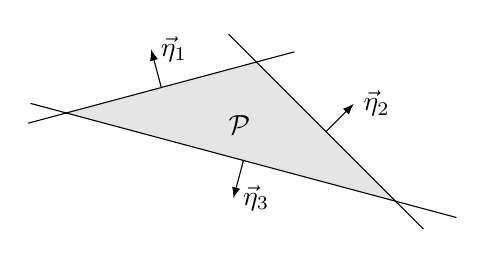
\begin{tikzpicture}
    \node at (0,0) {} coordinate(p1) ++(15:2.5) coordinate(p2) ++(-45:2.5) coordinate(p3) ++ (-195:4.0) coordinate(p4);
    \path[fill=gray!20] (p1) -- (p2) -- (p3);
    \node at (barycentric cs:p1=1,p2=1,p3=1) {$\mathcal{P}$};

    \foreach \X [count=\Y] in {2,...,4}
    {
      \path (p\Y) -- (p\X) coordinate[pos=-0.2](a\Y{}l) coordinate[pos=1.2](a\Y{}r) coordinate[pos=0.5](m\Y\X);
      \draw[-latex] (a\Y{}l) -- (m\Y\X) -- ([turn]90:.5) node[right]{$\vec{\eta}_\Y$};
      \draw (m\Y\X) -- (a\Y{}r);
    }
  \end{tikzpicture}
  \caption{A $3$-sided polyhedron.}\label{fig:triangle_inequality}
\end{figure}

Since we suppose there are at most the number of constraints as dimensions, it is not possible to create polyhedrons.
\end{document}
